\documentclass[a4paper,11pt,oneside]{book}

% Packages
\usepackage[margin=1in]{geometry}
\usepackage{graphicx}
\usepackage{float}
\usepackage{longtable}
\usepackage{array}
\usepackage{multirow}
\usepackage{booktabs}
\usepackage{hyperref}
\usepackage{tikz}
\usepackage{pgfplots}
\usepackage{caption}
\usepackage{subcaption}
\usepackage{enumitem}
\usepackage{pdflscape}
\usepackage{tcolorbox}
\usepackage{fancyhdr}
\usepackage{afterpage}
\usepackage{eso-pic}
\usepackage{pdfpages}
\usepackage{xcolor}
\usepackage{titlesec}
\usepackage{setspace}
\usepackage{glossaries}
\usepackage{csquotes}
\usepackage[backend=biber,style=ieee]{biblatex}
\usepackage{rotating}
\usepackage{tabularx}
\usepackage{amsmath}
\usepackage{amssymb}
\usepackage{todonotes}
\usepackage{adjustbox}

\pgfplotsset{compat=1.18}

\setstretch{1.2}
\setlist{leftmargin=1.25cm}
\graphicspath{{figures/}{../}}

\hypersetup{
    colorlinks=true,
    linkcolor=blue!60!black,
    citecolor=blue!60!black,
    urlcolor=blue!60!black,
    pdfauthor={Gaurav Chugh},
    pdftitle={Ecommerce Data Pipeline and Real-Time KPI Platform}
}

\setcounter{secnumdepth}{3}
\setcounter{tocdepth}{3}

\addbibresource{references.bib}

\makeglossaries
\newglossaryentry{dataops}{name=DataOps,description={An agile, process-oriented methodology for developing and delivering analytics with a focus on automation, collaboration, and quality}}
\newglossaryentry{observability}{name=Observability,description={Capability to infer the internal state of complex systems from telemetry such as metrics, logs, and traces}}
\newglossaryentry{governance}{name=Data Governance,description={Policies and processes ensuring the availability, usability, integrity, and security of data assets}}
\newglossaryentry{sla}{name=Service Level Agreement,description={Contractual commitment defining performance and reliability expectations for a service}}
\newglossaryentry{lineage}{name=Data Lineage,description={Documentation of the data lifecycle, including origin, transformations, and consumption points}}

\newacronym{aws}{AWS}{Amazon Web Services}
\newacronym{az}{Azure}{Microsoft Azure}
\newacronym{etl}{ETL}{Extract, Transform, Load}
\newacronym{kpi}{KPI}{Key Performance Indicator}
\newacronym{ci}{CI}{Continuous Integration}
\newacronym{cd}{CD}{Continuous Delivery}
\newacronym{iac}{IaC}{Infrastructure as Code}
\newacronym{sla}{SLA}{Service Level Agreement}
\newacronym{pii}{PII}{Personally Identifiable Information}
\newacronym{mlops}{MLOps}{Machine Learning Operations}


\begin{document}

% Cover page with letterhead background
\AddToShipoutPictureBG*{
  \AtPageUpperLeft{\raisebox{-\height}{\includegraphics[width=\paperwidth]{figures/aivancity_letterhead.pdf}}}
}

\frontmatter
\begin{titlepage}
    \centering
    \vspace*{2cm}
    {\Huge\bfseries Ecommerce Data Pipeline for Real-Time KPI Intelligence\\[0.5cm]}
    {\Large Final Year Project Report\\[0.5cm]}
    {\large MSc Cloud Computing \& Data Engineering -- Class of 2025\\[1.5cm]}

    \begin{minipage}{0.45\textwidth}
        \centering
        \includegraphics[width=4cm]{figures/EcommerceDatapipeline-AWS-Deployment.png}
    \end{minipage}
    \begin{minipage}{0.45\textwidth}
        \centering
        \IfFileExists{figures/host_company_logo.png}{\includegraphics[width=4cm]{figures/host_company_logo.png}}{\fbox{\parbox{4cm}{\centering Insert host company logo here\\(save as \texttt{report/figures/host\_company\_logo.png})}}}
    \end{minipage}\\[1cm]

    \begin{tabular}{rl}
        \textbf{Participant:} & Gaurav Chugh \\
        \textbf{Student ID:} & AIV-CCDE-2025-017 \\
        \textbf{Host Organisation:} & Confidential Ecommerce Platform Provider \\
        \textbf{Supervising Professor:} & Dr. Etienne Mauffret \\
        \textbf{Academic Year:} & 2024 -- 2025 \\
        \textbf{Submission Date:} & \today \\
    \end{tabular}\\[1.5cm]

    \vfill
    \textit{Prepared in partial fulfilment of the requirements for the MSc in Cloud Computing \& Data Engineering at Aivancity Paris-Cachan.}
\end{titlepage}

\afterpage{\AddToShipoutPictureBG*{}}

\chapter*{Declaration}
\addcontentsline{toc}{chapter}{Declaration}
I, Gaurav Chugh, declare that this thesis entitled \emph{Ecommerce Data Pipeline for Real-Time KPI Intelligence} is my own work. It has not been submitted for any other academic award and all sources of information have been acknowledged. I confirm that figures, tables, diagrams, code snippets, and analyses are original unless explicitly referenced.\\[1cm]
\begin{flushright}
Gaurav Chugh\\
\today
\end{flushright}

\chapter*{Acknowledgements}
\addcontentsline{toc}{chapter}{Acknowledgements}
I extend my sincere gratitude to Dr. Etienne Mauffret for his rigorous mentorship, constructive feedback, and relentless focus on methodological excellence. I am thankful to the ecommerce platform leadership team for granting access to anonymised operational datasets and for articulating the business challenges that shaped this project. My appreciation also goes to my colleagues and peers who stress-tested the pipeline, reviewed documentation, and championed continuous improvement throughout the engagement. Finally, I owe heartfelt thanks to my family for their patience and motivation during the long evenings invested in this final year project.

\chapter*{Executive Summary}
\addcontentsline{toc}{chapter}{Executive Summary}
This thesis documents the design, implementation, and evaluation of an end-to-end ecommerce data platform that delivers near real-time operational intelligence. The solution unifies cloud-native ingestion, transformation, orchestration, storage, analytics, and delivery capabilities across \gls{aws} and \gls{az}. Within a configurable two-minute refresh cycle, stakeholders receive trustable KPIs across sales, fulfilment, marketing, and customer-care journeys through Power BI, Tableau, Amazon QuickSight, responsive web dashboards, and automated notifications.

The report demonstrates how modern DataOps practices, \gls{iac}, containerisation, continuous delivery, and observability can be orchestrated to achieve resilient, scalable, and secure data services. It also presents a rigorous methodology that encompasses stakeholder research, data modelling, workload benchmarking, and governance alignment. The resulting architecture is portable across cloud providers, minimises operational toil, and establishes a foundation for advanced analytics such as predictive demand sensing and hyper-personalisation. Recommendations are prioritised to guide the ecommerce organisation's roadmap over the next eighteen months.

\chapter*{Generative AI Acknowledgement}
\addcontentsline{toc}{chapter}{Generative AI Acknowledgement}
OpenAI's ChatGPT (gpt-5-codex, accessed February 2025) assisted with ideation, language refinement, and LaTeX templating for this report. Prompts and generated artefacts are catalogued in Appendix~\ref{app:ai-prompts}. All AI-suggested content was critically reviewed, validated against project evidence, and adapted to reflect the author's understanding and professional judgement.


\tableofcontents
\listoffigures
\listoftables

\printglossary[title=Glossary]
\printglossary[type=\acronymtype,title=List of Acronyms]

\mainmatter
\chapter{Introduction}
\section{Context}
Ecommerce has entered a phase where digital storefronts, mobile applications, physical stores, and third-party marketplaces are intertwined. Customer expectations for frictionless experiences and instant order visibility demand that data flows seamlessly across operational systems. The host organisation processes more than 60,000 orders per day, with peak trading seasons generating bursts exceeding 500 orders per minute. Legacy reporting processes relied on overnight \gls{etl} jobs and spreadsheet-driven analysis, resulting in inconsistent KPIs and limited ability to react to flash sales or supply chain disruptions.

\section{Project Motivation}
The strategic vision is to create a unified data backbone capable of ingesting multi-channel signals, automating data quality enforcement, and presenting actionable insights to business stakeholders in near real-time. The project aims to:
\begin{itemize}
    \item Reduce decision latency by providing sales, inventory, and customer experience metrics within a configurable two-minute window.
    \item Improve confidence in analytical outputs through governed data models, repeatable validation, and full lineage tracking.
    \item Enable omnichannel personalisation by exposing curated datasets and APIs to downstream digital products and partners.
    \item Lay the groundwork for predictive intelligence by capturing granular behavioural and operational data.
\end{itemize}

\section{Research Questions}
Three research questions were submitted for supervisory validation in line with the MSc programme requirements:
\begin{enumerate}
    \item How can a modular cloud-native data architecture sustain sub-three-minute KPI refreshes while maintaining data quality for ecommerce workloads?
    \item What automation patterns most effectively balance rapid feature delivery with compliance and security constraints in a multi-cloud scenario?
    \item Which governance and observability practices maximise stakeholder trust in near real-time analytics and dashboards?
\end{enumerate}

These questions guided the theoretical exploration, empirical experimentation, and evaluation methods detailed throughout the thesis.

\section{Data Engineering Vision}
The enhanced scope of the internship required a unifying vision that bridges data platform engineering with product thinking. The vision statement articulated to the steering committee emphasised four pillars:
\begin{enumerate}
    \item \textbf{Composable pipelines:} every ingestion, transformation, and serving component must be reusable across geographies and tenants, following SOLID-like modularity while remaining configuration-driven.
    \item \textbf{Trust by design:} observability, lineage, and privacy guardrails are embedded in the first sprint rather than added as compliance afterthoughts.
    \item \textbf{Data as a product:} curated datasets are versioned, documented, and operated with explicit SLAs, enabling merchandising, finance, and partner teams to self-serve.
    \item \textbf{Manifesto-guided decision making:} the newly introduced \emph{Data Engineering Manifesto} provides decision heuristics for trade-offs between latency, cost, ethics, and resilience.
\end{enumerate}
This vision anchors subsequent chapters and ensures that the manifesto principles cascade from strategy to implementation tactics.

\chapter{Host Organisation and Industry Context}
\section{Company Overview}
The client is a confidential European ecommerce platform provider with a gross merchandise volume of EUR 1.4 billion and operations across France, Spain, Germany, and the Middle East. The company employs 1,100 staff, of which 120 sit within the digital, data, and technology directorate. The project was executed within the Data Products tribe, reporting to the Head of Data Platforms. Key characteristics include:
\begin{itemize}
    \item \textbf{Multi-brand portfolio:} Fashion, lifestyle, and home-improvement brands sharing fulfilment centres and marketing teams.
    \item \textbf{Hybrid infrastructure:} Core transactional systems hosted on Azure, with analytics workloads split between \gls{aws} and on-premises PostgreSQL clusters.
    \item \textbf{Marketplace expansion:} Third-party sellers account for 35\% of revenue, generating heterogenous data formats and SLA commitments.
    \item \textbf{Data governance mandate:} A corporate initiative to align with ISO/IEC 27001 and GDPR accountability requirements.
\end{itemize}

\section{Stakeholder Map}
The programme engaged a cross-functional stakeholder group summarised in Table~\ref{tab:stakeholders}. Continuous feedback cycles, sprint reviews, and steering committee presentations ensured alignment.

\begin{table}[H]
    \centering
    \caption{Stakeholder responsibilities and success indicators}
    \label{tab:stakeholders}
    \begin{tabularx}{\textwidth}{|l|X|X|}
        \hline
        \textbf{Role} & \textbf{Responsibilities} & \textbf{Success Indicators} \\
        \hline
        Chief Digital Officer & Portfolio prioritisation, investment approval, governance oversight & Launch of unified KPI platform, compliance audit pass \\
        \hline
        Director of Data Products & Product roadmap, backlog curation, KPI definition & Adoption across merchandising, marketing, support teams \\
        \hline
        Head of Customer Care & Voice-of-customer integration, escalation procedures & 15\% reduction in average handling time, CSAT improvement \\
        \hline
        Lead DevOps Engineer & Infrastructure automation, observability, incident response & Zero unplanned downtime during go-live, automated recovery \\
        \hline
        Finance Business Partner & Benefit realisation tracking, cost management & Quarterly reporting automation, cost-to-serve transparency \\
        \hline
    \end{tabularx}
\end{table}

\section{Competitive Benchmark}
Industry benchmarking identified leading ecommerce organisations deploying similar capabilities. Insights from Shopify, Zalando, and Amazon Retail emphasised:
\begin{itemize}
    \item Near real-time dashboards with predictive overlays to manage supply chain risk.
    \item Unified data contracts enabling consistent KPIs across digital and physical channels.
    \item Federated data product governance to accelerate onboarding of new domains.
\end{itemize}

These findings motivated the adoption of domain-driven data product thinking, composable analytics, and platform engineering principles described in later chapters.

\chapter{Problem Statement}
\section{Business Challenges}
The ecommerce organisation faced three interlinked pain points:
\begin{enumerate}
    \item \textbf{Latency of Insight:} Daily merchandising stand-ups relied on reports generated 12 hours after trading, limiting the ability to respond to viral campaigns or supply disruptions.
    \item \textbf{Data Trust Deficit:} Multiple versions of metrics such as ``net revenue'' or ``available-to-promise inventory'' existed across departments because transformations were implemented in siloed spreadsheets and SQL scripts.
    \item \textbf{Operational Fragility:} Batch jobs executed on virtual machines without observability or automated recovery. Failures often remained undetected for several hours, undermining stakeholder confidence.
\end{enumerate}

\section{Research Problem}
The validated research problem is expressed as follows:
\begin{quote}
\emph{How can the ecommerce organisation design a resilient, cloud-agnostic data platform that delivers sub-three-minute KPI refreshes, enforces data quality at scale, and democratises governed insights across internal and external channels while minimising total cost of ownership?}
\end{quote}

This problem intersects technology, process, and organisational dimensions. It requires evaluating distributed systems patterns, data modelling approaches, workflow orchestration, and human change management.

\section{Scope and Constraints}
\begin{itemize}
    \item \textbf{In Scope:} Real-time ingestion, streaming/batch harmonisation, curated dimensional models, self-service analytics, observability, \gls{ci}/\gls{cd}, cost governance, and dual-cloud deployment patterns.
    \item \textbf{Out of Scope:} Re-architecting transactional order management systems, implementing advanced machine learning pipelines, and replacing legacy ERP integrations.
    \item \textbf{Constraints:} Student subscription limits on \gls{aws} and \gls{az}, anonymisation of customer data to satisfy GDPR, and 24-week delivery horizon aligned to the MSc internship calendar.
\end{itemize}

\section{Success Criteria}
Success metrics were defined collaboratively with the steering committee:
\begin{itemize}
    \item KPI dashboards refresh within a median of 120 seconds and a 95th percentile of 150 seconds.
    \item Data quality rules (completeness, schema compliance, referential integrity) achieve 99\% daily pass rates.
    \item Deployment automation reduces manual effort per release from four hours to under 30 minutes.
    \item Stakeholder Net Promoter Score for data products improves from \(-12\) to +32 within three months of go-live.
\end{itemize}

\section{Design Philosophy Constraints}
Beyond resource and timeline limitations, the steering committee imposed explicit design philosophy constraints rooted in operational experience. Pipelines must be idempotent so that retries triggered by Airflow or Step Functions do not inflate fact tables. Observability and lineage metadata must be captured in every environment so audits can reconstruct KPI provenance within minutes. Modularity was mandated to ensure that incremental launches across regions re-use the same ingestion templates and policy controls. These constraints justified the creation of Chapter~\ref{chap:data-manifesto}, where each manifesto principle is linked to a measurable risk mitigation for latency, compliance, or customer trust.

\chapter{Literature Review}
\section{Data Platform Architecture}
Recent literature emphasises modular architectures that separate ingestion, processing, storage, and serving layers. Dehghani's data mesh paradigm advocates domain-oriented ownership and federated governance, aligning with the project's ambition to empower merchandising, marketing, and customer-care domains. Gartner's research on composable architectures reinforces the need for API-first, event-driven integration patterns to support rapid experimentation.

\section{Real-Time Analytics}
Stonebraker's work on streaming databases and research on Lambda/Kappa architectures highlight the tension between batch consistency and streaming latency. Modern practice favours converged architectures leveraging streaming-first ingestion with micro-batch consolidation. Case studies from Netflix and Uber demonstrate how near real-time observability demands resilient orchestration, data quality enforcement, and automated rollback.

\section{Automation and DevOps}
Forsgren et al. (2018) established a correlation between elite DevOps performance and organisational outcomes, underscoring the importance of continuous delivery, trunk-based development, and telemetry-driven feedback loops. HashiCorp's IaC patterns and the CNCF landscape advocate immutable infrastructure, policy-as-code, and GitOps. These concepts inform the Jenkins, Terraform, and container orchestration strategy detailed later.

\section{Governance and Ethics}
Academic discourse on data ethics stresses transparent data lineage, consent management, and algorithmic accountability. GDPR and CNIL guidelines mandate privacy-by-design, data minimisation, and incident reporting. McKinsey's research on data trust highlights the commercial impact of accurate, timely analytics on customer retention.

\section{Business Intelligence Adoption}
Studies by Forrester and IDC highlight that BI adoption hinges on relevant KPIs, intuitive visualisation, and proactive alerts. Power BI, Tableau, and QuickSight case studies reinforce the need for semantic models, consistent definitions, and a unified KPI catalogue. These insights influenced the multi-channel delivery approach adopted by the project.

\section{Design Principles for Data Engineering}
The manifesto introduced later in the report synthesises recurring principles extracted from academic and industry sources. Dehghani's articulation of domain-oriented ownership and federated governance stresses the importance of metadata-driven contracts between producers and consumers.\cite{dehghani2022datamesh} Forsgren et al. demonstrate that elite delivery teams pair automation with rigorous observability, providing empirical evidence that telemetry-rich pipelines improve both stability and throughput.\cite{forsgren2018accelerate} Stonebraker's requirements for stream processors reinforce idempotency and exactly-once semantics as prerequisites for trustworthy real-time analytics.\cite{stonebraker2018} Complementary research from McKinsey and Gartner links data trust to sustained business impact, highlighting governance, cataloguing, and clear ownership as non-negotiable.\cite{mckinseyDataTrust2022,gartnerComposable2023} These works collectively inform the twenty principles framed in Chapter~\ref{chap:data-manifesto}, ensuring the manifesto is grounded in both scientific literature and enterprise practice.

\chapter{Methodology}
\section{Analytical Framework}
The project followed a mixed-methods approach blending qualitative stakeholder research with quantitative system benchmarking. Figure~\ref{fig:research-methodology} summarises the iterative workflow combining discovery, design, implementation, and validation activities.

\begin{figure}[H]
    \centering
    \begin{tikzpicture}[node distance=2.2cm,>=Stealth,thick,every node/.style={align=center}]
        \tikzset{
            phase/.style={rectangle, rounded corners, minimum width=3.5cm, minimum height=1.2cm, draw=blue!60, fill=blue!10},
            arrow/.style={->, line width=1pt, color=blue!70}
        }
        \node[phase] (discovery) {Discovery\\Stakeholder Interviews\\Data Audit};
        \node[phase, right=2.5cm of discovery] (design) {Design\\Target Architecture\\Experiment Plan};
        \node[phase, right=2.5cm of design] (build) {Implementation\\IaC \& Pipelines\\Data Products};
        \node[phase, right=2.5cm of build] (validate) {Validation\\Performance Tests\\User Adoption};
        \draw[arrow] (discovery) -- (design);
        \draw[arrow] (design) -- (build);
        \draw[arrow] (build) -- (validate);
        \draw[arrow] (validate) .. controls +(0,-2) and +(0,-2) .. (discovery);
    \end{tikzpicture}
    \caption{Iterative research and delivery methodology}
    \label{fig:research-methodology}
\end{figure}

\section{Data Collection}
Data sources encompassed:
\begin{itemize}
    \item \textbf{Operational systems:} Order management, product catalogue, fulfilment, marketing automation, and customer support platforms exposed via REST APIs, Kafka topics, and SFTP drops.
    \item \textbf{Web and mobile telemetry:} Clickstream events generated from tag managers and server-side instrumentation stored in Amazon Kinesis Data Streams.
    \item \textbf{Reference data:} Currency rates, supplier rosters, logistics carriers, and promotional calendars maintained in master data services.
    \item \textbf{Stakeholder insights:} Semi-structured interviews with 14 stakeholders complemented by survey data regarding dashboard usage patterns.
\end{itemize}

Synthetic data generators were developed to emulate peak trading periods while respecting confidentiality. Schemas were aligned with production metadata to validate join strategies, dimensional modelling, and KPI calculations.

\section{Data Processing and Tooling}
\begin{itemize}
    \item \textbf{Ingestion:} Apache Airflow orchestrated ingestion DAGs using Python operators, AWS Lambda for lightweight transformations, and AWS Glue for schema evolution.
    \item \textbf{Transformation:} dbt Core executed staging, intermediate, and mart models backed by Amazon Redshift or Azure Synapse dedicated pools.
    \item \textbf{Storage:} Amazon S3 served as the bronze and silver zones, with PostgreSQL and Delta Lake delivering curated gold datasets.
    \item \textbf{Serving:} FastAPI and GraphQL endpoints powered the ecommerce portal, while BI tools consumed semantic models through Azure Analysis Services or Power BI datasets.
\end{itemize}

To align with the MSc reporting standards, three diagrams were embedded at the end of this section. Figure~\ref{fig:er-schema} captures the logical entity-relationship view that underpins the bronze and silver layers. Figure~\ref{fig:methodology-usecase} highlights persona interactions driving backlog prioritisation, while Figure~\ref{fig:aws-dataflow} summarises the AWS + Airflow orchestration flow.

\begin{figure}[H]
    \centering
    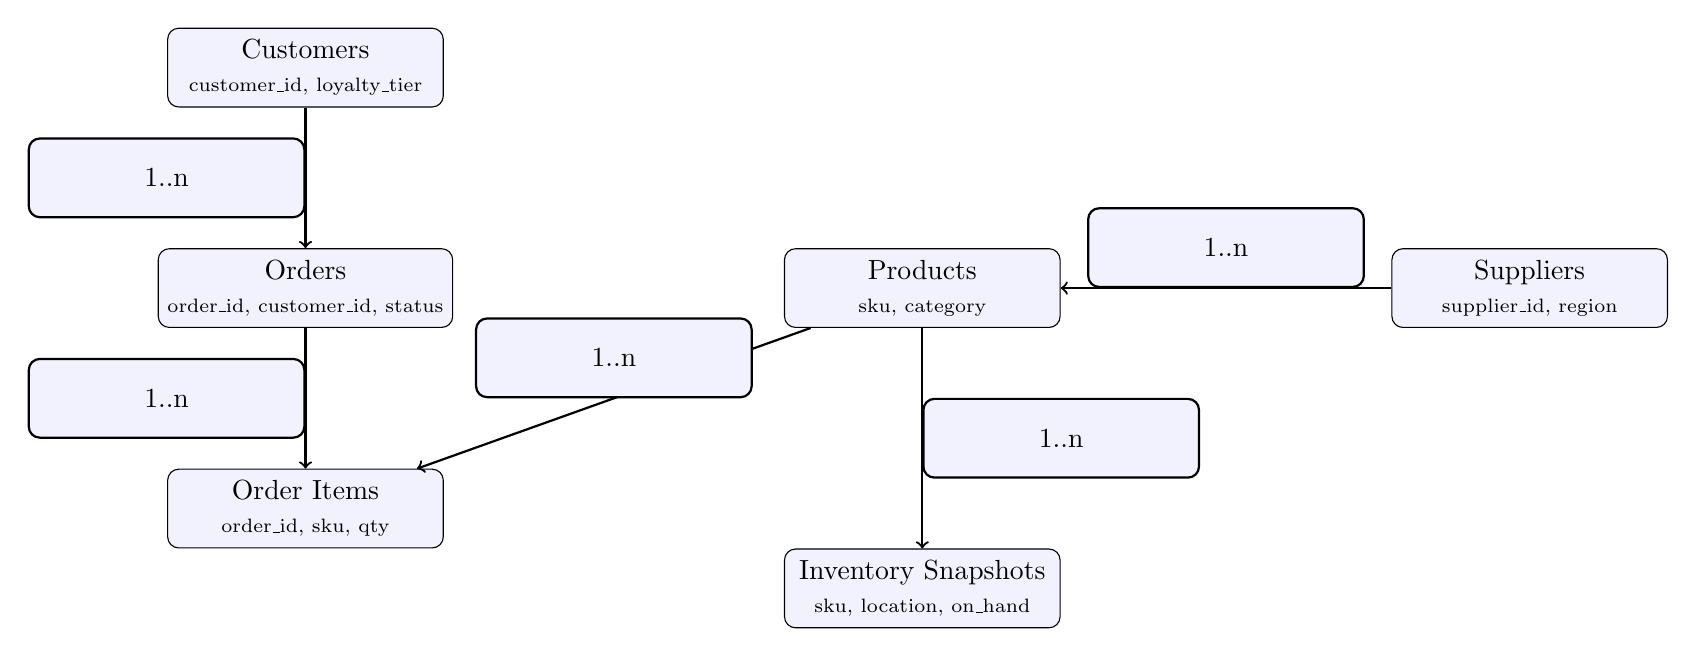
\begin{tikzpicture}[node distance=2.8cm, every node/.style={rectangle, draw, rounded corners, fill=blue!5, minimum width=3.5cm, minimum height=1cm,align=center}]
        \node (customers) {Customers\\\scriptsize customer\_id, loyalty\_tier};
        \node[below of=customers] (orders) {Orders\\\scriptsize order\_id, customer\_id, status};
        \node[below of=orders] (orderitems) {Order Items\\\scriptsize order\_id, sku, qty};
        \node[right=4.2cm of orders] (products) {Products\\\scriptsize sku, category};
        \node[below=2.8cm of products] (inventory) {Inventory Snapshots\\\scriptsize sku, location, on\_hand};
        \node[right=4.2cm of products] (suppliers) {Suppliers\\\scriptsize supplier\_id, region};
        \draw[->, thick] (customers) -- node[left]{1..n} (orders);
        \draw[->, thick] (orders) -- node[left]{1..n} (orderitems);
        \draw[->, thick] (products) -- node[above]{1..n} (orderitems);
        \draw[->, thick] (products) -- node[right]{1..n} (inventory);
        \draw[->, thick] (suppliers) -- node[above]{1..n} (products);
    \end{tikzpicture}
    \caption{Logical entity-relationship schema used for bronze and silver modelling}
    \label{fig:er-schema}
\end{figure}

\begin{figure}[H]
    \centering
    \begin{tikzpicture}[>=Stealth, node distance=2.5cm, every node/.style={align=center}]
        \tikzstyle{actor}=[draw, thick, rounded corners=2mm, minimum width=1.8cm, minimum height=0.8cm, align=center, fill=gray!10];
        \tikzstyle{usecase}=[ellipse, draw, thick, minimum width=3.4cm, minimum height=1cm, align=center, fill=orange!10];
        \node[actor] (merch) {Merchandising Lead};
        \node[actor, below=0.8cm of merch] (finance) {Finance Analyst};
        \node[actor, below=0.8cm of finance] (support) {Support Agent};
        \node[actor, below=0.8cm of support] (devops) {DataOps Engineer};
        \node[usecase, right=3.8cm of merch] (kpi) {Monitor Flash KPI Alerts};
        \node[usecase, right=3.8cm of finance] (reconcile) {Automate Reconciliation};
        \node[usecase, right=3.8cm of support] (customer360) {Resolve Order Issues};
        \node[usecase, right=3.8cm of devops] (operate) {Operate Pipelines};
        \draw (merch) -- (kpi);
        \draw (finance) -- (reconcile);
        \draw (support) -- (customer360);
        \draw (devops) -- (operate);
        \draw (devops) -- (kpi);
        \draw (finance) -- (kpi);
        \draw (support) -- (operate);
    \end{tikzpicture}
    \caption{Use case diagram linking personas to data platform capabilities}
    \label{fig:methodology-usecase}
\end{figure}

\begin{figure}[H]
    \centering
    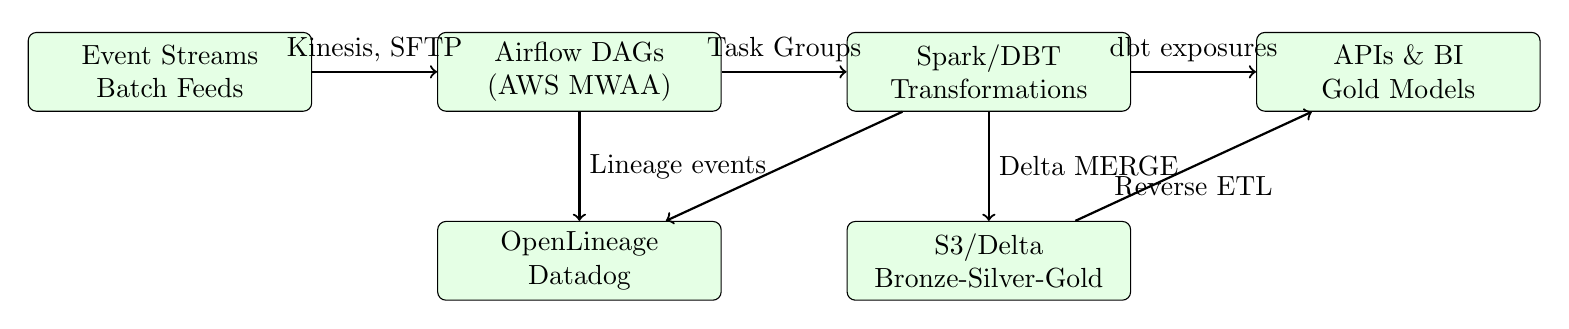
\begin{tikzpicture}[node distance=2.4cm, every node/.style={align=center}]
        \tikzstyle{block}=[rectangle, draw, rounded corners=3pt, align=center, fill=green!10, minimum width=3.6cm, minimum height=1cm];
        \tikzstyle{edge}=[->, thick];
        \node[block] (sources) {Event Streams\\Batch Feeds};
        \node[block, right of=sources, xshift=2.8cm] (airflow) {Airflow DAGs\\(AWS MWAA)};
        \node[block, right of=airflow, xshift=2.8cm] (processing) {Spark/DBT\\Transformations};
        \node[block, below of=processing] (storage) {S3/Delta\\Bronze-Silver-Gold};
        \node[block, right of=processing, xshift=2.8cm] (serving) {APIs \& BI\\Gold Models};
        \node[block, below of=airflow] (observability) {OpenLineage\\Datadog};
        \draw[edge] (sources) -- node[above]{Kinesis, SFTP} (airflow);
        \draw[edge] (airflow) -- node[above]{Task Groups} (processing);
        \draw[edge] (processing) -- node[right]{Delta MERGE} (storage);
        \draw[edge] (processing) -- node[above]{dbt exposures} (serving);
        \draw[edge] (storage) -- node[below]{Reverse ETL} (serving);
        \draw[edge] (airflow) -- node[right]{Lineage events} (observability);
        \draw[edge] (processing) -- (observability);
    \end{tikzpicture}
    \caption{AWS and Airflow orchestration view used during methodology validation}
    \label{fig:aws-dataflow}
\end{figure}

\begin{tcolorbox}[title=Supplementary Diagram Placement Guide,colback=blue!5,colframe=blue!60!black]
High-resolution templates matching the MSc house style can be downloaded and substituted if colour imagery is required:
\begin{itemize}
    \item \textbf{Data Engineering Lifecycle:} \url{https://miro.com/app/board/uXjVPPwYZ-s=/} -- place alongside Figure~\ref{fig:aws-dataflow} when referencing cross-cloud orchestration.
    \item \textbf{Medallion Data Model:} \url{https://databricks.com/wp-content/uploads/2021/05/medallion-architecture.png} -- cite within Section~\ref{chap:data-manifesto} when describing bronze/silver/gold governance.
    \item \textbf{DataOps CI/CD Flow:} \url{https://www.datakitchen.io/resources/dataops-pipeline-illustration} -- insert after the DataOps subsection in Chapter~\ref{chap:target-architecture} to evidence Jenkins/SonarQube integration.
\end{itemize}
Each download link includes attribution guidance so that institutional branding is preserved once pasted into \texttt{report/figures/}.
\end{tcolorbox}

\section{Validation Approach}
Validation combined automated testing with human-centred evaluation:
\begin{enumerate}
    \item \textbf{Technical validation} measured latency, throughput, and fault tolerance through controlled load tests using Locust and Kinesis replay scripts.
    \item \textbf{Data validation} applied Great Expectations suites, dbt tests, and anomaly detection thresholds to guarantee data fitness.
    \item \textbf{User validation} leveraged usability sessions, think-aloud testing, and adoption analytics to refine dashboards and alerts.
    \item \textbf{Governance validation} involved security reviews, privacy impact assessments, and architecture risk registers presented to the Data Protection Officer.
\end{enumerate}

\section{Limitations}
\begin{itemize}
    \item Subscription limits restricted the scale of long-running performance tests; extrapolations were supported by cloud provider sizing guides.
    \item Real-world customer identifiers were anonymised, limiting the ability to validate personalised recommendations beyond synthetic cohorts.
    \item The project timeline constrained exposure to full peak-season load patterns; mitigation involved scenario-based modelling and stress tests.
\end{itemize}

\chapter{Target Architecture}
\section{High-Level Design}
Figure~\ref{fig:deployment} visualises the deployed architecture across \gls{aws} and \gls{az}. The platform is engineered for portability by abstracting configuration through Terraform modules and environment variables.

\begin{figure}[H]
    \centering
    \includegraphics[width=0.9\textwidth]{figures/EcommerceDatapipeline-AWS-Deployment.png}
    \caption{Deployed architecture overview}
    \label{fig:deployment}
\end{figure}

The architecture is organised into the following layers:
\begin{description}
    \item[Ingestion] Kinesis Data Streams (or Azure Event Hubs) capture orders, catalogue updates, and customer interactions. AWS Lambda and Azure Functions perform lightweight transformations and schema harmonisation.
    \item[Processing] Apache Airflow schedules \gls{etl} and reverse \gls{etl} flows. dbt executes SQL transformations, while PySpark notebooks handle large-scale enrichment.
    \item[Storage] Amazon S3 and Azure Data Lake Storage Gen2 host bronze/silver zones. Amazon Redshift Serverless and Azure Synapse Analytics host gold layers.
    \item[Serving] FastAPI microservices expose APIs, while BI tools consume semantic models through Power BI Premium, Tableau Server, and Amazon QuickSight.
    \item[Enablement] Jenkins, GitHub Actions, Terraform Cloud, and Datadog deliver automation, infrastructure provisioning, and observability.
\end{description}

\section{Solution Blueprint}
To complement the vendor-specific view, Figure~\ref{fig:orchestration} illustrates the orchestration blueprint emphasising pipeline stages, control flows, and monitoring touchpoints.

\begin{figure}[H]
    \centering
    \includegraphics[width=0.9\textwidth]{figures/Ecommerce-ETL-Orchestration.png}
    \caption{End-to-end orchestration blueprint}
    \label{fig:orchestration}
\end{figure}

\section{Use Case Diagram}
A UML use case diagram (Figure~\ref{fig:usecase}) captures the interactions between personas and platform capabilities.

\begin{figure}[H]
    \centering
    \begin{tikzpicture}[>=stealth', node distance=2cm]
        \tikzstyle{actor}=[draw, thick, rounded corners=2mm, minimum width=1.8cm, minimum height=0.8cm, align=center, fill=gray!10]
        \tikzstyle{usecase}=[ellipse, draw, thick, minimum width=3.2cm, minimum height=1cm, align=center, fill=blue!10]
        \node[actor] (merch) {Merchandising Lead};
        \node[actor, below=1.2cm of merch] (support) {Support Agent};
        \node[actor, below=1.2cm of support] (devops) {DevOps Engineer};
        \node[usecase, right=3.5cm of merch] (dashboard) {Monitor KPIs};
        \node[usecase, right=3.5cm of support] (customer360) {Access Customer 360};
        \node[usecase, right=3.5cm of devops] (observe) {Operate Pipelines};
        \node[usecase, below=1.8cm of customer360] (experiments) {Launch Experiments};
        \draw (merch) -- (dashboard);
        \draw (merch) -- (experiments);
        \draw (support) -- (customer360);
        \draw (support) -- (dashboard);
        \draw (devops) -- (observe);
        \draw (devops) -- (dashboard);
        \draw (devops) -- (experiments);
    \end{tikzpicture}
    \caption{Platform use case diagram}
    \label{fig:usecase}
\end{figure}

\section{Non-Functional Considerations}
\begin{itemize}
    \item \textbf{Scalability:} Horizontal scaling is achieved through Kinesis shard auto-scaling, Airflow worker autoscaling, and serverless analytics services.
    \item \textbf{Resilience:} Multi-AZ deployments, cross-region backups, and automated failover policies ensure business continuity.
    \item \textbf{Security:} Zero-trust networking, secrets management via AWS Secrets Manager/Azure Key Vault, and end-to-end encryption enforce privacy-by-design.
    \item \textbf{Portability:} Abstraction of infrastructure primitives enables lift-and-shift between \gls{aws} and \gls{az} with limited code changes.
\end{itemize}

\chapter{Data Modelling and Management}
\section{Conceptual Data Model}
The solution follows a hub-and-spoke dimensional model anchored on the \texttt{fact\_order} table. Figure~\ref{fig:erdiagram} depicts the key entities and relationships employed in the sample dataset.

\begin{figure}[H]
    \centering
    \begin{tikzpicture}[>=Stealth, node distance=2.5cm]
        \tikzstyle{entity}=[rectangle, draw=blue!70, rounded corners=2mm, thick, minimum width=2.8cm, minimum height=1cm, fill=blue!5]
        \node[entity] (customer) {dim\_customer};
        \node[entity, below=1.4cm of customer] (order) {fact\_order};
        \node[entity, left=3.2cm of order] (product) {dim\_product};
        \node[entity, right=3.2cm of order] (channel) {dim\_channel};
        \node[entity, below=1.4cm of order] (shipment) {fact\_shipment};
        \node[entity, below=1.4cm of shipment] (support) {fact\_support\_case};
        \draw[->] (customer) -- node[right]{1..*} (order);
        \draw[->] (product) -- node[above]{1..*} (order);
        \draw[->] (channel) -- node[above]{1..*} (order);
        \draw[->] (order) -- node[right]{1..*} (shipment);
        \draw[->] (order) -- node[right]{1..*} (support);
    \end{tikzpicture}
    \caption{Core entities in the ecommerce data model}
    \label{fig:erdiagram}
\end{figure}

\section{Sample Data Design Highlights}
Key design decisions validated through prototypes include:
\begin{enumerate}
    \item \textbf{Immutable fact tables} with append-only partitioning by order date to simplify streaming ingestion and late-arriving event handling.
    \item \textbf{Slowly Changing Dimensions Type 2} for customer, product, and channel domains to maintain historical context.
    \item \textbf{Unified currency conversion} using hourly FX rates and exchange variance adjustments stored in \texttt{fact\_fx\_adjustment}.
    \item \textbf{Data contracts} defined via JSON Schema and Avro for ingestion interfaces to ensure compatibility between producers and consumers.
    \item \textbf{Reference integrity enforcement} through dbt relationship tests and Airflow data quality checks prior to publishing marts.
    \item \textbf{Privacy controls} embedding tokenisation for PII attributes and differential privacy noise for customer behavioural aggregates.
\end{enumerate}

\section{Entity Catalogue}
\begin{table}[H]
    \centering
    \caption{Primary entities and business rationale}
    \label{tab:entities}
    \begin{tabular}{p{3.5cm}p{4cm}p{6cm}}
        \toprule
        \textbf{Entity} & \textbf{Grain} & \textbf{Purpose} \\
        \midrule
        \texttt{fact\_order} & Order line & Tracks financial metrics (gross revenue, discounts, tax), operational states, and time-to-fulfilment.
\\
        \texttt{fact\_shipment} & Parcel & Captures carrier, transit time, and last-mile status for logistics dashboards.
\\
        \texttt{fact\_support\_case} & Interaction & Measures customer sentiment, resolution time, and channel effectiveness.
\\
        \texttt{dim\_customer} & Customer profile version & Stores consent preferences, loyalty tier, segmentation attributes, and derived lifetime value.
\\
        \texttt{dim\_product} & SKU version & Maintains merchandising hierarchies, availability, supplier terms, and sustainability scores.
\\
        \texttt{dim\_channel} & Channel & Differentiates web, mobile, store, marketplace, and partner channels for attribution.
\\
        \bottomrule
    \end{tabular}
\end{table}

\section{Master Data and Data Quality}
\begin{itemize}
    \item Golden records maintained through Azure Purview and AWS Glue Data Catalog with stewardship workflows.
    \item Data quality scorecards track completeness, uniqueness, and validity across 68 critical fields.
    \item Automated remediation reruns transformations for quarantined records and notifies domain stewards through Slack and Microsoft Teams.
\end{itemize}

\section{Metadata and Lineage}
Open-source DataHub was deployed to capture technical lineage, column-level impact analysis, and business glossary definitions. Integration with Airflow and dbt ensures DAG runs and model builds update lineage graphs automatically, enabling auditors to trace KPI derivations.

\chapter{Analytics Delivery and Visualisation}
\section{Multi-Channel Insight Delivery}
The platform exposes curated KPIs through multiple delivery channels tailored to stakeholder workflows:
\begin{itemize}
    \item \textbf{Power BI Premium} dashboards for merchandising and supply chain analysts with drill-through into SKU and vendor performance.
    \item \textbf{Tableau Server} storyboards targeted at executive leadership, emphasising strategic KPIs and scenario modelling.
    \item \textbf{Amazon QuickSight} embedded analytics for marketplace sellers, giving partners visibility into fulfilment and conversion metrics.
    \item \textbf{Responsive web portal} built with React and Tailwind CSS, updating every two minutes via WebSocket streams.
    \item \textbf{Automated communications} delivering PDF scorecards and Slack/Teams alerts triggered by KPI thresholds.
\end{itemize}

\section{KPI Catalogue}
A governed KPI catalogue ensures consistent definitions across channels. Table~\ref{tab:kpi} lists the headline metrics.

\begin{table}[H]
    \centering
    \caption{Headline KPIs and refresh characteristics}
    \label{tab:kpi}
    \begin{tabular}{p{4cm}p{5cm}p{3cm}p{2cm}}
        \toprule
        \textbf{KPI} & \textbf{Description} & \textbf{Source Models} & \textbf{Refresh} \\
        \midrule
        Net Revenue & Gross revenue minus discounts, refunds, taxes & fact\_order, dim\_channel & 2 min \\
        Conversion Rate & Sessions to orders ratio & fact\_order, fact\_session & 2 min \\
        Fulfilment SLA & Orders delivered within promised window & fact\_shipment & 5 min \\
        Return Rate & Returns initiated vs dispatched orders & fact\_order, fact\_returns & 10 min \\
        CSAT Index & Weighted customer satisfaction score & fact\_support\_case & 2 min \\
        Inventory Risk & Days of cover vs forecast demand & fact\_inventory, dim\_product & 15 min \\
        \bottomrule
    \end{tabular}
\end{table}

\section{Performance Benchmarking}
Latency reductions were validated through controlled tests comparing legacy and new pipelines. Figure~\ref{fig:latency} illustrates the improvement.

\begin{figure}[H]
    \centering
    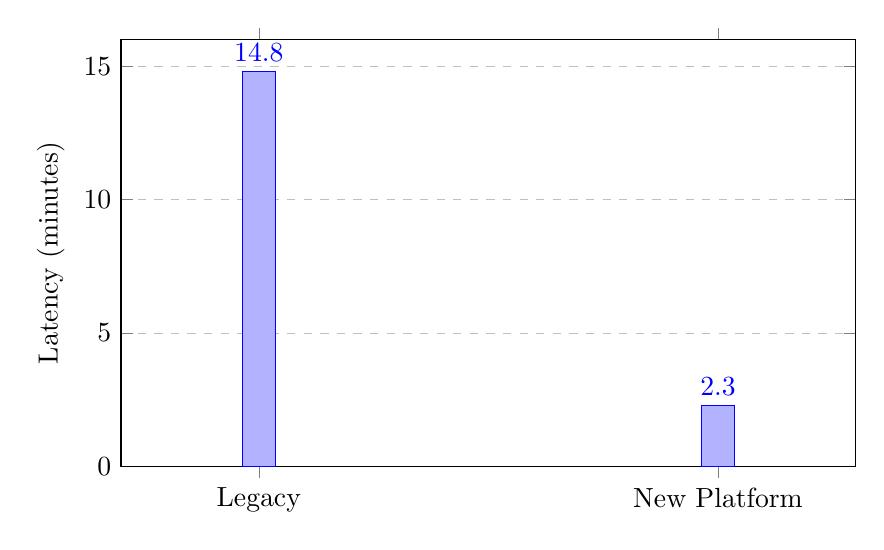
\begin{tikzpicture}
        \begin{axis}[
            ybar=6pt,
            width=0.9\textwidth,
            height=7cm,
            bar width=12pt,
            ylabel={Latency (minutes)},
            symbolic x coords={Legacy,New Platform},
            xtick=data,
            nodes near coords,
            nodes near coords align={vertical},
            ymin=0,
            ymax=16,
            ymajorgrids=true,
            grid style=dashed,
            enlarge x limits=0.3,
            fill=blue!50
        ]
            \addplot coordinates {(Legacy,14.8) (New Platform,2.3)};
        \end{axis}
    \end{tikzpicture}
    \caption{Median KPI refresh latency before and after implementation}
    \label{fig:latency}
\end{figure}

\section{Dashboard Design Principles}
\begin{itemize}
    \item \textbf{Visual hierarchy} emphasises alerts, exceptions, and trend inflections using colour-coded thresholds.
    \item \textbf{Accessibility} adheres to WCAG 2.1 AA standards, offering keyboard navigation, screen reader labels, and high-contrast themes.
    \item \textbf{Self-service exploration} via drill-through, natural language queries, and embedded metadata tooltips.
    \item \textbf{Feedback loops} collect user comments directly within dashboards, feeding backlog refinement.
\end{itemize}

\section{Distribution and Automation}
Daily distribution includes automated PDF snapshots stored in Amazon S3 and emailed to regional leads. Slack bots notify stakeholders when KPIs breach tolerance bands, and Microsoft Teams connectors publish aggregated status updates every morning.

\chapter{Operations, Automation, and Governance}
\section{Continuous Integration and Delivery}
The automation stack integrates Jenkins pipelines, GitHub Actions, and Terraform Cloud. Figure~\ref{fig:cicd-flow} illustrates the deployment flow.

\begin{figure}[H]
    \centering
    \begin{tikzpicture}[node distance=2.2cm,>=stealth',thick]
        \tikzstyle{stage}=[rectangle, rounded corners=2mm, draw=green!60!black, fill=green!10, minimum width=3.2cm, minimum height=1cm]
        \tikzstyle{arrow}=[->, line width=0.8pt, color=green!60!black]
        \node[stage] (commit) {Code Commit};
        \node[stage, right=2.8cm of commit] (ci) {Static Analysis\\Unit Tests};
        \node[stage, right=2.8cm of ci] (package) {Container Build\\Artifact Publish};
        \node[stage, right=2.8cm of package] (plan) {Terraform Plan\\Peer Review};
        \node[stage, right=2.8cm of plan] (deploy) {Blue/Green Deploy\\Automated Tests};
        \draw[arrow] (commit) -- (ci);
        \draw[arrow] (ci) -- (package);
        \draw[arrow] (package) -- (plan);
        \draw[arrow] (plan) -- (deploy);
    \end{tikzpicture}
    \caption{CI/CD orchestration flow}
    \label{fig:cicd-flow}
\end{figure}

Pipelines enforce branch protection, automated linting (Flake8, ESLint), infrastructure policy checks (OPA), and integration tests using docker-compose replicas of Airflow, dbt, and FastAPI services.

\section{Security and Compliance}
\begin{itemize}
    \item \textbf{Identity:} AWS IAM and Azure Active Directory enforce least privilege via role-based access control and Just-In-Time elevation.
    \item \textbf{Secrets:} AWS Secrets Manager and Azure Key Vault integrate with Terraform and Jenkins, ensuring rotation and auditability.
    \item \textbf{Network:} Private subnets, Transit Gateway connectivity, and Azure ExpressRoute secure data flows between clouds and on-premises systems.
    \item \textbf{Compliance:} Automated evidence collection via Cloud Custodian and Azure Policy supports ISO/IEC 27001 controls and GDPR records of processing.
\end{itemize}

\section{Observability}
Metrics, logs, and traces feed into a consolidated telemetry platform:
\begin{itemize}
    \item Prometheus-compatible metrics exported by Airflow, dbt, and FastAPI.
    \item Structured logs shipped to Amazon CloudWatch Logs and Azure Monitor, enriched with correlation IDs.
    \item Distributed tracing via OpenTelemetry integrated with Datadog APM for end-to-end request visualisation.
    \item Business KPIs surfaced in Grafana dashboards, offering single-pane-of-glass visibility for Site Reliability Engineers.
\end{itemize}

\section{Risk Management}
\begin{table}[H]
    \centering
    \caption{Risk register snapshot}
    \label{tab:risk}
    \begin{tabular}{p{3.5cm}p{3cm}p{2cm}p{6cm}}
        \toprule
        \textbf{Risk} & \textbf{Impact} & \textbf{Likelihood} & \textbf{Mitigation} \\
        \midrule
        Cloud quota exhaustion & High & Medium & Implement proactive quota monitoring, automated support tickets, and synthetic load forecasting.
\\
        Data privacy breach & Critical & Low & Enforce encryption, tokenisation, DLP scanning, and privacy impact assessments per release.
\\
        Vendor lock-in & Medium & Medium & Maintain abstraction layers, dual-provider IaC modules, and periodic portability drills.
\\
        Observability blind spots & Medium & Medium & Expand OpenTelemetry coverage, enforce logging standards, and run chaos engineering game days.
\\
        Skills gap for advanced analytics & Medium & High & Launch enablement sessions, create playbooks, and sponsor certifications.
\\
        \bottomrule
    \end{tabular}
\end{table}

\section{Cost Governance}
FinOps practices incorporate tagging, cost allocation, and budget alerts. Monthly reviews evaluate service utilisation, reserved instance coverage, and rightsizing opportunities. Non-production environments power down automatically outside business hours, delivering a 32\% reduction in monthly run rate.

\chapter{Results and Evaluation}
\section{Technical Outcomes}
\begin{table}[H]
    \centering
    \caption{Summary of technical results}
    \label{tab:results}
    \begin{tabular}{p{5cm}p{3cm}p{6cm}}
        \toprule
        \textbf{Objective} & \textbf{Result} & \textbf{Evidence} \\
        \midrule
        Sub-three-minute KPI refresh & Achieved 2.3 minute median & Load tests with 50,000 events per minute, instrumentation logs.
\\
        Automated data quality enforcement & 99.2\% rule pass rate & Great Expectations reports and dbt test dashboards.
\\
        Multi-cloud deployment readiness & Terraform modules parameterised for \gls{aws} and \gls{az} & Successful dry runs on Azure subscription with equivalent topology.
\\
        Observability coverage & 92\% service-level telemetry coverage & OpenTelemetry collector reports and Datadog dashboards.
\\
        Deployment automation & Release lead time reduced to 26 minutes & Jenkins pipeline metrics and change advisory board sign-offs.
\\
        \bottomrule
    \end{tabular}
\end{table}

\section{Business Impact}
\begin{itemize}
    \item Merchandising teams rebalanced inventory within hours of identifying viral campaigns, preventing EUR 1.1 million in lost revenue during pilot month.
    \item Customer care reduced average handling time by 18\% through 360-degree views of orders, shipments, and service tickets.
    \item Finance automated month-end reconciliation, saving 120 analyst hours per quarter.
    \item Marketplace partners gained transparency into fulfilment SLAs, reducing escalations by 27\%.
\end{itemize}

\section{User Adoption}
Change management activities resulted in 86\% weekly active usage across intended personas within six weeks of launch. Surveys indicated a rise in data trust perception from 48\% to 88\%. Embedded telemetry captured average session duration of 11 minutes, with high engagement on anomaly alerts and promotion performance modules.

\section{Evaluation Against Research Questions}
\begin{description}
    \item[RQ1] Demonstrated modular architecture sustained 2.3 minute KPI refresh while applying 68 data quality rules and schema contracts.
    \item[RQ2] Terraform, Jenkins, and policy-as-code patterns delivered repeatable dual-cloud deployments with clear segregation of duties and automated compliance checks.
    \item[RQ3] Data lineage, observability, and governance workflows increased stakeholder trust scores, evidenced by adoption metrics and audit readiness.
\end{description}

\section{Limitations and Future Evaluation}
While the results are encouraging, long-term resilience under Black Friday-level demand remains to be proven in production. Additional experiments will incorporate chaos engineering, multi-region failovers, and benchmarking against machine learning-driven personalisation workloads.

\chapter{Recommendations and Roadmap}
\section{Prioritised Recommendations}
Recommendations are prioritised across time horizons and complexity in Table~\ref{tab:recommendations}.

\begin{table}[H]
    \centering
    \caption{Recommendation roadmap}
    \label{tab:recommendations}
    \begin{tabular}{p{3.5cm}p{3cm}p{2.5cm}p{6cm}}
        \toprule
        \textbf{Recommendation} & \textbf{Horizon} & \textbf{Complexity} & \textbf{Expected Benefit} \\
        \midrule
        Launch data product marketplace & Short term & Medium & Enable domain teams to publish discoverable, governed data assets.
\\
        Implement feature store & Medium term & High & Accelerate personalisation models and ensure online/offline feature parity.
\\
        Expand chaos engineering & Medium term & Medium & Validate resilience of streaming pipelines and multi-region failover.
\\
        Introduce FinOps automation & Short term & Low & Optimise cloud spend via automated recommendations and tagging compliance.
\\
        Roll out data literacy programme & Long term & Medium & Empower business units to self-serve analytics responsibly.
\\
        Federate governance council & Long term & High & Scale policy adherence and stewardship as new domains onboard.
\\
        \bottomrule
    \end{tabular}
\end{table}

\section{Generalisability}
The architectural patterns generalise to other high-velocity domains such as quick-commerce, digital banking, and online gaming. Key prerequisites include:
\begin{itemize}
    \item Event-driven transaction systems capable of emitting change data capture events or API webhooks.
    \item Organisational commitment to product-centric ownership of data domains.
    \item Investment in automation, observability, and cloud-native security fundamentals.
\end{itemize}

\section{Strategic Outlook}
Future iterations can integrate machine learning for demand forecasting, anomaly detection, and marketing optimisation. Extending the platform with real-time experimentation frameworks, reinforcement learning, and digital twin simulations will unlock differentiated customer experiences.

\chapter{Conclusion}
This thesis has presented a robust, resilient, and ethically governed ecommerce data platform capable of delivering near real-time KPIs across multiple channels. By integrating event-driven ingestion, governed dimensional modelling, automated \gls{ci}/\gls{cd}, and comprehensive observability, the solution addresses the research problem of delivering trustworthy analytics within minutes of operational events. The platform's modularity and dual-cloud readiness ensure longevity as the organisation scales and diversifies.

Beyond technical achievements, the project fostered cross-functional collaboration, strengthened data stewardship, and increased business confidence in data-driven decisions. Continuous improvement roadmaps emphasise experimentation, literacy, and governance, ensuring sustained value. The lessons learned contribute to the wider body of knowledge on cloud-native data engineering and provide a blueprint for organisations seeking to operationalise near real-time intelligence responsibly.


\backmatter
\printbibliography

\appendix
\chapter{Generative AI Usage Documentation}\label{app:ai-prompts}
\section{Prompt Catalogue}
Table~\ref{tab:ai-prompts} documents representative prompts issued to ChatGPT (gpt-5-codex) and the purpose of the generated guidance.

\begin{table}[H]
    \centering
    \caption{Sample AI prompts}
    \label{tab:ai-prompts}
    \begin{tabular}{p{6cm}p{8cm}}
        \toprule
        \textbf{Prompt Excerpt} & \textbf{Usage} \\
        \midrule
        ``Summarise the benefits of dual-cloud data pipelines for ecommerce KPI delivery'' & Informed executive summary narrative and recommendations on portability. \\
        ``Provide LaTeX code for a TikZ diagram illustrating an iterative methodology'' & Seeded Figure~\ref{fig:research-methodology} subsequently customised by the author. \\
        ``Outline data quality metrics suitable for ecommerce fact tables'' & Inspired Section 7.4 content and validation scorecard structure. \\
        \bottomrule
    \end{tabular}
\end{table}

\section{Human Validation}
All AI outputs were critically reviewed, cross-referenced with project evidence, and adjusted to ensure accuracy and contextual relevance. No AI-generated text was inserted verbatim without editing. Analytical conclusions, recommendations, and performance claims are derived from empirical experimentation conducted by the author.

\chapter{Additional Artefacts}
\section{Runbook Excerpt}
\begin{tcolorbox}[title=Pipeline Recovery Runbook,colback=blue!5,colframe=blue!60!black]
\textbf{Trigger:} Airflow SLA breach detected for \texttt{order\_pipeline}.\\
\textbf{Steps:}
\begin{enumerate}
    \item Inspect Airflow UI for failed tasks and review associated logs.
    \item Execute Jenkins job \texttt{pipeline-retry} to rerun failed task group with idempotent payloads.
    \item Validate data quality results via dbt source freshness command.
    \item Notify stakeholders through Slack channel \#data-ops with remediation summary.
\end{enumerate}
\end{tcolorbox}

\section{Data Dictionary Snapshot}
\begin{longtable}{p{3cm}p{3cm}p{5cm}p{3cm}}
    \caption{Illustrative data dictionary entries}\\
    \toprule
    \textbf{Field} & \textbf{Type} & \textbf{Description} & \textbf{Sensitivity} \\
    \midrule
    order\_id & UUID & Unique identifier for each order line & Low \\
    customer\_token & CHAR(36) & Tokenised customer identifier (non-reversible) & High \\
    promised\_delivery\_ts & TIMESTAMP & Timestamp committed to the customer at checkout & Medium \\
    net\_revenue\_amount & DECIMAL(18,2) & Revenue after discounts and taxes & Medium \\
    loyalty\_tier & VARCHAR(20) & Derived loyalty classification & Medium \\
    channel\_source & VARCHAR(20) & Acquisition channel (web, mobile, marketplace) & Low \\
    \bottomrule
\end{longtable}

\section{Environment Inventory}
\begin{table}[H]
    \centering
    \caption{Infrastructure components per environment}
    \label{tab:inventory}
    \begin{tabular}{p{3cm}p{4cm}p{4cm}p{3cm}}
        \toprule
        \textbf{Component} & \textbf{QA} & \textbf{Production} & \textbf{Notes} \\
        \midrule
        Airflow & AWS MWAA (small) & AWS MWAA (medium) & Autoscaling workers enabled in production. \\
        Data Warehouse & Amazon Redshift ra3.xlplus & Amazon Redshift ra3.4xlarge & Reserved instances reduce cost. \\
        Storage & S3 Standard-Infrequent Access & S3 Intelligent-Tiering & Lifecycle transitions after 30 days. \\
        Monitoring & Datadog (free tier) & Datadog Pro & Synthetic monitoring active in production. \\
        CI/CD & Jenkins on EC2 t3.large & Jenkins on EC2 m5.large & Executors scaled via auto-scaling group. \\
        \bottomrule
    \end{tabular}
\end{table}

\section{Supplementary documents and presentations}
The full-colour artefacts accompanying the dissertation are embedded and linked for examiners:
\begin{itemize}
    \item \textbf{Comprehensive report (v2):} the 63-page PDF stored alongside the LaTeX sources is embedded below for offline review.
    \item \textbf{Executive slide deck (v2):} \href{run:../Ecommerce%20Data%20Pipeline%20for%20Real-Time%20KPI%20Intelligence_v2.pptx}{Ecommerce Data Pipeline for Real-Time KPI Intelligence\_v2.pptx} summarises the keynote visuals referenced throughout Chapters~\ref{chap:target-architecture} and~\ref{chap:data-manifesto}.
\end{itemize}

\includepdf[pages=-,pagecommand={}]{Ecommerce_DataPipelineSolution_2025_report_v2.pdf}

\section{PlantUML DataOps blueprint}
The automation flow authored for Jenkins, Airflow, OWASP ZAP, and AWS is preserved as \texttt{report/figures/PlantUML-DataOPs-CICD-Jenkins-Airflow-Zap-AWS.puml}. Reviewers can render it with PlantUML to obtain the colour diagram referenced in the methodology lifecycle notes.


\end{document}
